\begin{frame}
  \myheading{Module 6.1 : Eigenvalues and Eigenvectors}
\end{frame}

% Slide 2
\begin{frame}
  \begin{columns}
    \column{.5\textwidth}
    \begin{overlayarea}{\textwidth}{\textheight}
      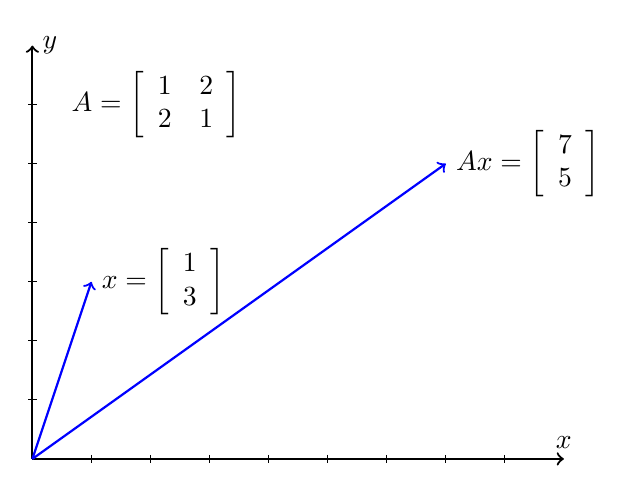
\begin{tikzpicture}[scale=0.75]
  \draw [thick, black, ->] (0,0) -- (9,0)
  node [above, black] {$x$};

  \draw [thick, black, ->] (0,0) -- (0,7)
  node [right, black] {$y$};

  \draw [thick, blue, ->] (0,0) -- (1,3)
  node [right, black] {$x = \left[ \begin{array}{c}
          1 \\
          3
        \end{array} \right]$};

  \draw (0.5,6)
  node [right, black] {$A = \left[ \begin{array}{cc}
          1 & 2 \\
          2 & 1
        \end{array} \right]$};

  \onslide<3->{
    \draw [thick, blue, ->] (0,0) -- (7,5)
    node [right, black] {$Ax = \left[ \begin{array}{c}
            7 \\
            5
          \end{array} \right]$};
  }
  \foreach \x/\xtext in {1/1,2/2,3/3,4/4,5,5,6/6,7/7,8/8 }
    {
      \draw[shift={(\x,0)}] (0pt, 2pt) -- (0pt, -2pt);
    }
  \foreach \y/\ytext in {1/1,2/2,3/3,4/4,5,5,6/6}{
      \draw[shift={(0,\y)}] (2pt, 0pt) -- (-2pt, 0pt);
    }
\end{tikzpicture}
    \end{overlayarea}
    \column{0.5\textwidth}
    \begin{overlayarea}{\textwidth}{\textheight}
      \only<1->{
        \begin{itemize}\justifying
          \item<1-> What happens when a matrix hits a vector?
          \item<2-> The vector gets transformed into a new vector (it strays from its path)
          \item<4-> The vector may also get scaled (elongated or shortened) in the process.
        \end{itemize}
      }
    \end{overlayarea}
  \end{columns}
\end{frame}

% Slide 3
\begin{frame}
  \begin{columns}
    \column{.5\textwidth}
    \begin{overlayarea}{\textwidth}{\textheight}
      \only<1-2>{\input{./modules/Module1/tikz_images/eigenvector_before_product.tex}}
      \only<3-> {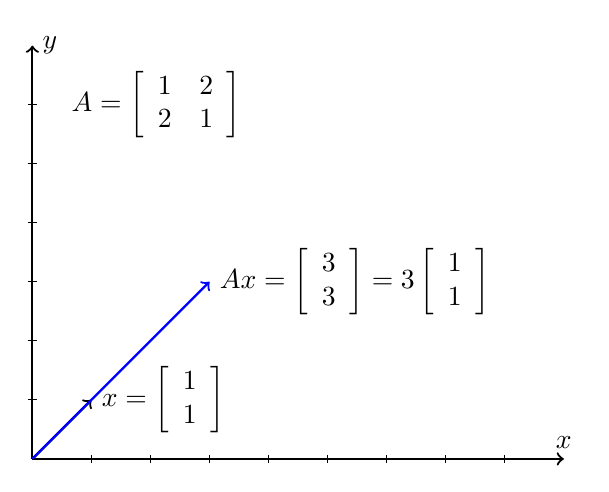
\begin{tikzpicture}[scale=0.75]
  \draw [thick, black, ->] (0,0) -- (9,0)
  node [above, black] {$x$};

  \draw [thick, black, ->] (0,0) -- (0,7)
  node [right, black] {$y$};

  \draw [thick, black, ->] (0,0) -- (1,1)
  node [right, black] {$x = \left[ \begin{array}{c}
          1 \\
          1
        \end{array} \right]$};

  \draw (0.5,6)
  node [right, black] {$A = \left[ \begin{array}{cc}
          1 & 2 \\
          2 & 1
        \end{array} \right]$};

  \draw [thick, blue, ->] (0,0) -- (3,3)
  node [right, black] {$Ax = \left[ \begin{array}{c}
          3 \\
          3
        \end{array} \right] = 3\left[ \begin{array}{c}
          1 \\
          1
        \end{array}
        \right]$};

  \foreach \x/\xtext in {1/1,2/2,3/3,4/4,5,5,6/6,7/7,8/8 }
    {
      \draw[shift={(\x,0)}] (0pt, 2pt) -- (0pt, -2pt); %node [below] {$\xtext$};
    }
  \foreach \y/\ytext in {1/1,2/2,3/3,4/4,5,5,6/6}{
      \draw[shift={(0,\y)}] (2pt, 0pt) -- (-2pt, 0pt); % node [left] {$\ytext$};
    }

\end{tikzpicture}
}
    \end{overlayarea}


    \column{0.5\textwidth}
    \begin{overlayarea}{\textwidth}{\textheight}
      \only<1->{
        \begin{itemize}\justifying
          \item<1-> For a given square matrix $A$, there exist special vectors which refuse to stray from their path.
          \item<4-> These vectors are called eigenvectors.
          \item<5-> More formally,
                \[
                  Ax = \lambda x \text{    [direction remains the same]}
                \]
          \item<6-> The vector will only get scaled but will not change its direction.
        \end{itemize}
      }
    \end{overlayarea}
  \end{columns}
\end{frame}

% Slide 4
\begin{frame}
  \begin{columns}
    \column{.5\textwidth}
    \begin{overlayarea}{\textwidth}{\textheight}
      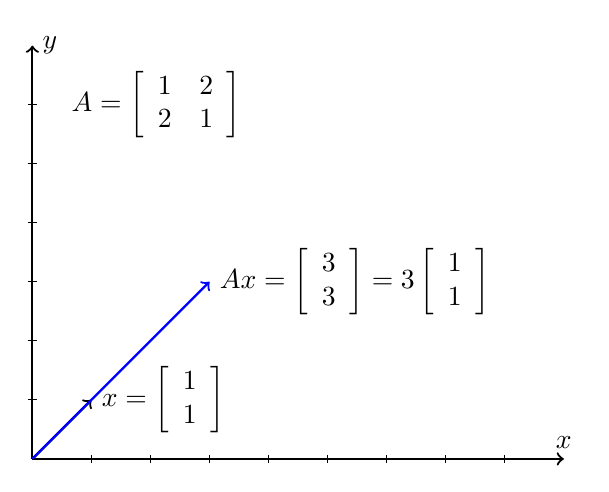
\begin{tikzpicture}[scale=0.75]
  \draw [thick, black, ->] (0,0) -- (9,0)
  node [above, black] {$x$};

  \draw [thick, black, ->] (0,0) -- (0,7)
  node [right, black] {$y$};

  \draw [thick, black, ->] (0,0) -- (1,1)
  node [right, black] {$x = \left[ \begin{array}{c}
          1 \\
          1
        \end{array} \right]$};

  \draw (0.5,6)
  node [right, black] {$A = \left[ \begin{array}{cc}
          1 & 2 \\
          2 & 1
        \end{array} \right]$};

  \draw [thick, blue, ->] (0,0) -- (3,3)
  node [right, black] {$Ax = \left[ \begin{array}{c}
          3 \\
          3
        \end{array} \right] = 3\left[ \begin{array}{c}
          1 \\
          1
        \end{array}
        \right]$};

  \foreach \x/\xtext in {1/1,2/2,3/3,4/4,5,5,6/6,7/7,8/8 }
    {
      \draw[shift={(\x,0)}] (0pt, 2pt) -- (0pt, -2pt); %node [below] {$\xtext$};
    }
  \foreach \y/\ytext in {1/1,2/2,3/3,4/4,5,5,6/6}{
      \draw[shift={(0,\y)}] (2pt, 0pt) -- (-2pt, 0pt); % node [left] {$\ytext$};
    }

\end{tikzpicture}

    \end{overlayarea}

    \column{0.5\textwidth}
    \begin{overlayarea}{\textwidth}{\textheight}
      \only<2->{
        \begin{itemize}\justifying
          \item<2-> So what is so special about eigenvectors?
          \item<3-> Why are they always in the limelight?
          \item<4-> It turns out that several properties of matrices can be analyzed based
                on their eigenvalues (for example, see spectral graph theory)
          \item<5-> We will now see two cases where eigenvalues/vectors will help us in this
                course
        \end{itemize}
      }
    \end{overlayarea}
  \end{columns}
\end{frame}

% Slide 5
\begin{frame}
  \begin{columns}
    \column{0.35\textwidth}
    %\only<2->{
    \onslide<2->
    \begin{center}
      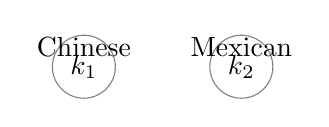
\begin{tikzpicture}
        \draw [color=black!50](0,0) circle(0.4) node [black] {$k_1$} node [black,above=0.3]{Chinese};
        \draw [color=black!50](2,0) circle(0.4) node [black] {$k_2$} node [black,above=0.3]{Mexican};
      \end{tikzpicture}
    \end{center}
    \[
      v_{(0)} = \left[ \begin{array}{c}
          k_1 \\
          k_2
        \end{array} \right]
    \]
    \onslide<5->
    \begin{equation*}
      \begin{aligned}
        v_{(1)}       & = \left[ \begin{array}{c}
            pk_1 + (1 - q)k_2 \\
            (1 - p)k_1 + qk_2
          \end{array} \right] \\
        \onslide<6->{ & = \left[ \begin{array}{cc}
              p     & 1 - q \\
              1 - p & q
            \end{array} \right]
          \left[ \begin{array}{c}
              k_1 \\
              k_2
            \end{array} \right]}
      \end{aligned}
    \end{equation*}
    %}
    %\only<6->{
    \onslide<7->
    \begin{equation*}
      \begin{aligned}
        v_{(1)} & = & M v_{(0)}   \\
        v_{(2)} & = & M v_{(1)}   \\
                & = & M^2 v_{(0)}
      \end{aligned}
    \end{equation*}
    %}
    %\only<7->{
    \onslide<8->
    In general, $v_{(n)} = M^n v_{(0)}$
    %}

    \column{0.65\textwidth}
    \begin{overlayarea}{\textwidth}{\textheight}
      %\only<1->{
      \begin{itemize}\justifying
        \onslide<1-> \item Let us assume that on day $0$, $k_1$ students eat Chinese food,
              and $k_2$ students eat Mexican food. (Of course, no one eats in the mess!)
              \onslide<3-> \item On each subsequent day $i$, a fraction $p$ of the students who ate
              Chinese food on day $(i-1)$, continue to eat Chinese food on day $i$, and $(1-p)$
              shift to Mexican food.
              \onslide<4-> \item Similarly a fraction $q$ of students who ate Mexican food on day $(i-1)$
              continue to eat Mexican food on day $i$, and $(1-q)$ shift to Chinese food.
              \onslide<8-> \item The number of customers in the two restaurants is thus given by the
              following series:
              \[
                v_{(0)}, Mv_{(0)}, M^2v_{(0)}, M^3v_{(0)}, \dots
              \]
      \end{itemize}
      %}
    \end{overlayarea}
  \end{columns}
\end{frame}


% Slide 6
\begin{frame}
  \begin{columns}
    \column{0.4\textwidth}
    \begin{overlayarea}{\textwidth}{\textheight}
      \vspace{1in}
      \begin{center}
        \begin{tikzpicture}[>=stealth',shorten >=1pt,auto,node distance=2cm]
  \node[state] (k1) {$k_1$};
  \node[state] (k2) [right of=k1] {$k_2$};

  \path[->] (k1) edge [loop left] node {$p$} (k1)
  edge [bend left=60]  node  {$1-p$} (k2)
  (k2)  edge [loop right] node {$q$} (k2)
  edge [bend left=60] node  {$1-q$} (k1);
\end{tikzpicture}

      \end{center}
    \end{overlayarea}
    \column{0.6\textwidth}
    \begin{overlayarea}{\textwidth}{\textheight}
      \only<2->{
        \begin{itemize}\justifying
          \item<2-> This is a problem for the two restaurant owners.
          \item<3-> The number of patrons is changing constantly.
          \item<4-> Or is it? Will the system eventually reach a
                steady state? (i.e. will the number of customers in
                the two restaurants become constant over time?)
          \item<5-> Turns out they will!
          \item<6-> Let's see how?
        \end{itemize}
      }
    \end{overlayarea}
  \end{columns}
\end{frame}

% Slide 7
\begin{frame}
  \begin{columns}
    \column{0.4\textwidth}
    \begin{overlayarea}{\textwidth}{\textheight}
      \only<1->{
        \begin{block}{Definition}
          Let $\lambda_1, \lambda_2, \dots, \lambda_n$ be the eigenvectors
          of an $n\times n$ matrix $A$. $\lambda_1$ is called the dominant eigen
          value of $A$ if
          \begin{equation*}
            |\lambda_1| \geq |\lambda_i| \text{  } i = 2, \dots , n
          \end{equation*}
        \end{block}
      }
      \only<3->{
        \begin{block}{Theorem}
          The largest (dominant) eigenvalue of a stochastic matrix is 1.
          \newpage
          \href{https://yutsumura.com/eigenvalues-of-a-stochastic-matrix-is-always-less-than-or-equal-to-1/}{See proof here}
        \end{block}
      }
    \end{overlayarea}
    \column{0.6\textwidth}
    \begin{overlayarea}{\textwidth}{\textheight}
      \only<2->{
        \begin{block}{Definition}
          \justifying
          A matrix $M$ is called a stochastic matrix if all the entries are positive
          and the sum of the elements in each column is equal to $1$.
          \newline
          (Note that the matrix in our example is a stochastic matrix)
        \end{block}
      }
      \only<4->{
        \begin{block}{Theorem}
          \justifying
          If $A$ is a $n \times n$ square matrix with a dominant eigenvalue, then the sequence
          of vectors given by $Av_0$, $A^2v_0$, $\dots,$ $A^nv_0, \dots$ approaches a multiple of the
          dominant eigenvector of $A$.
          \newline
          (the theorem is slightly misstated here for ease of explanation)
        \end{block}
      }
    \end{overlayarea}
  \end{columns}
\end{frame}

% Slide 8
\begin{frame}
  \begin{columns}
    \column{0.6\textwidth}
    \begin{overlayarea}{\textwidth}{\textheight}
        \begin{itemize}\justifying
          \item<1-> Let $e_d$ be the dominant eigenvector of $M$ and $\lambda_d = 1$ the corresponding dominant eigenvalue
          \item<2-> Given the previous definitions and theorems, what can
                you say about the sequence $Mv_{(0)}, M^2v_{(0)}, M^3v_{(0)}, \dots $?
          \item<3-> There exists an $n$ such that
                \begin{equation*}
                  v_{(n)} = M^nv_{(0)} = ke_d \text{ (some multiple of $e_d$)}
                \end{equation*}
          \item<4-> Now what happens at time step $(n+1)$?
                \begin{equation*}
                  \hspace{-0.28in}
                  v_{(n+1)} = Mv_{(n)} = M(ke_d) = k(Me_d) = k(\lambda_d e_d) = ke_d
                \end{equation*}
          \item<5-> The population in the two restaurants becomes constant after
                time step $n$. \\
                \href{https://www.quora.com/Why-does-repeatedly-multiplying-a-vector-by-a-square-matrix-cause-the-vector-to-converge-on-or-along-the-matrixs-eigenvector}{See Proof Here}
        \end{itemize}
    \end{overlayarea}

    \column{0.4\textwidth}
    \begin{overlayarea}{\textwidth}{\textheight}
    \begin{center}
      \begin{tikzpicture}[>=stealth',shorten >=1pt,auto,node distance=2cm]
  \node[state] (k1) {$k_1$};
  \node[state] (k2) [right of=k1] {$k_2$};

  \path[->] (k1) edge [loop left] node {$p$} (k1)
  edge [bend left=60]  node  {$1-p$} (k2)
  (k2)  edge [loop right] node {$q$} (k2)
  edge [bend left=60] node  {$1-q$} (k1);
\end{tikzpicture}

    \end{center}
    \end{overlayarea}
  \end{columns}
\end{frame}

% Slide 9
\begin{frame}
  \begin{overlayarea}{\textwidth}{\textheight}
    \begin{itemize}\justifying
      \item Now instead of a stochastic matrix let us consider any square matrix $A$
      \item<2-> Let $p$ be the time step at which the sequence $x_0, Ax_0, A^2x_0, \dots$ approaches a multiple of $e_d$ (the dominant eigenvector of $A$)
            \onslide<3-> {
              \begin{align*}
                \onslide<3-> {A^px_0     & = ke_d \\}
                \onslide<4-> {A^{p+1}x_0 & = A (A^px_0) = kAe_d = k\lambda_de_d \\}
                \onslide<5-> {A^{p+2}x_0 & = A (A^{p+1}x_0) = k\lambda_dAe_d = k\lambda_d^2e_d \\}
                \onslide<6-> {A^{p+n}x_0 & =} \onslide<7-> {k(\lambda_d)^ne_d}
              \end{align*}
            }
      \item<8-> In general, if $\lambda_d$ is the dominant eigenvalue of a matrix $A$,
            what would happen to the sequence $x_0, Ax_0, A^2x_0, \dots$ if
            \begin{itemize}\justifying
              \item<9-> $|\lambda_d| > 1$ \visible<10->{(will explode)}
              \item<11-> $|\lambda_d| < 1$ \visible<12->{(will vanish)}
              \item<13-> $|\lambda_d| = 1$ \visible<14->{(will reach a steady state)}
            \end{itemize}
      \item<15-> (We will use this in the course at some point)
    \end{itemize}
  \end{overlayarea}
\end{frame}
